% !Mode:: "TeX:UTF-8"
%\documentclass[twocolumn]{sig-alternate}
%\documentclass[letterpaper, twocolumn]{sig-alt-hotnetscr}
%\documentclass{hotnets15}
%\documentclass[letterpaper, twocolumn]{sig-alternate-10pt}
%\documentclass[twocolumn,10pt]{infocom}
%\documentclass[twocolumn,10pt]{IEEEtran_v15}
%\documentclass[twocolumn,10pt]{IEEEtran}
%\documentclass[twocolumn,10pt]{article}
%\usepackage[sort,nocompress,space]{cite}
%\documentclass[letterpaper,twocolumn,10pt]{article}
%\usepackage{usenix,epsfig,endnotes}
%\usepackage[letterpaper]{geometry}
\documentclass[letterpaper,twocolumn,10pt]{article}
\usepackage{usenix,epsfig,endnotes}

\usepackage{ifpdf}
\usepackage{balance}
%\usepackage[T1]{fontenc}
%\usepackage{raged2e}
\ifpdf
\setlength{\pdfpagewidth}{8.5in}
\setlength{\pdfpageheight}{11in}
\else
\fi

%%%%%%%%%%%%%%%%%%%%%%
% Set Compact Mode   %
%%%%%%%%%%%%%%%%%%%%%%

%\newcommand{\subparagraph}{}


%\usepackage[compact]{titlesec}
%\titlespacing{\section}{0pt}{*0}{*0}
%\titlespacing{\subsection}{0pt}{*0}{*0}
%\titlespacing{\subsubsection}{0pt}{*0}{*0}
%\setlength{\parskip}{0pt}
%\setlength{\parsep}{0pt}
%\setlength{\headsep}{0pt}
%\setlength{\topskip}{0pt}
%\setlength{\topmargin}{0pt}
%\setlength{\topsep}{0pt}
%\setlength{\partopsep}{0pt}
%\setlength{\itemsep}{0pt}

%%%%%%%%%%%%%%%%%%%%%%
%
%%%%%%%%%%%%%%%%%%%%%%


\usepackage{url}
\usepackage[sort,space]{cite}
\usepackage{lineno}
\renewcommand\linenumberfont{\normalfont\bfseries\small}
\usepackage{pifont}
%\usepackage{times}
%\usepackage[activate={true,nocompatibility}]{microtype}
\usepackage{epsfig,epsf,url,amssymb}
\usepackage{tabularx}
%\usepackage{algorithm2e}
\usepackage[ruled,vlined]{algorithm2e}
\usepackage{algpseudocode}
\usepackage{amsmath}
\usepackage{amsthm}
\usepackage{mathtools}
\newtheorem{mydef}{Definition}
\usepackage{rotating}
\usepackage{wrapfig}
\usepackage{times}
\long\def\comment#1{}
\usepackage{multirow}
\usepackage{enumitem}
\usepackage{lscape}
\usepackage{stmaryrd}
\usepackage{wrapfig}
\usepackage{hhline}
\usepackage{textcomp,booktabs}
\usepackage[usenames,dvipsnames]{color}
\usepackage{colortbl}
\usepackage{multirow}
\usepackage{rotating}
\usepackage{epstopdf}
\definecolor{mygray}{gray}{.9}
\definecolor{mypink}{gray}{.9}
\definecolor{mycyan}{cmyk}{.3,0,0,0}

\usepackage{graphicx}
%\usepackage{subfigure}
\usepackage{subfig}
\usepackage[font=bf]{caption}

\newcommand{\bbR}{\mathbb{R}}
\newcommand{\calN}{\mathcal{N}}
\newcommand{\calR}{\mathcal{R}}
\newcommand{\calV}{\mathcal{V}}
\newcommand{\eg}{{\it e.g.}}
\newcommand{\etal}{{\it et al.~}}
\newcommand{\etc}{{\it etc.}}
\newcommand{\ie}{{\it i.e.}}
\newcommand{\tablecapspace}{{\vspace{-0.1in}}}
\newcommand{\tablespace}{{\vspace{-0.05in}}}
\newcommand{\picspace}{{\vspace{-0.1in}}}
\renewcommand{\baselinestretch}{1}
\renewcommand{\arraystretch}{1.05}      % make the space between tabular lines larger
\newcommand{\capspace}{}           % control space between figure/table and caption

\def\TODO#1{\textcolor{red}{#1}}



%\setlength{\textheight}{9.3in}
%\setlength{\columnsep}{1.4pc}
%\setlength{\textwidth}{7.1in}

\newcommand{\ignore}[1]{{}}
\newcommand{\sys}{{CODA}\xspace}
\newcommand{\abs}{{DNA}\xspace}
\newcommand{\hong}{\textcolor{black}}


\newcommand{\paragraphb}[1]{\vspace{0.05in}\noindent{\bf #1}}
\newtheorem{my}{Heuristic}
\newtheorem{you}{Proposition}
\newtheorem{observation}{Observation}

\newcommand{\paraspace}{\vspace{0.05in}}
\newcommand{\parab}[1]{\paraspace\noindent{\bf #1} }
\newcommand{\parae}[1]{\paraspace\noindent{\em #1} }
\newcommand{\parabe}[1]{\paraspace\noindent{\bf \em #1} }
\newcommand{\kai}[1]{{\color{red}[Kai: #1]}}
\def\naive{na\"\i ve}



\newcommand{\tabincell}[2]{\begin{tabular}{@{}#1@{}}#2\end{tabular}}

\newcommand{\subcaption}[1]{\centerline{#1}\vspace{0.1in}}
\long\def\comment#1{}
\newtheorem{theorem}{Theorem}
\newtheorem{lemma}[theorem]{Lemma}
\newtheorem{proposition}[theorem]{Proposition}
\newtheorem{corollary}[theorem]{Corollary}
%\newtheorem{problem}[theorem]{Problem}

\newenvironment{definition}[1][Definition]{\begin{trivlist}
\item[\hskip \labelsep {\bfseries #1}]}{\end{trivlist}}
\newenvironment{problem}[1][]{\begin{trivlist}
\item[\hskip \labelsep {\bfseries}]}{\end{trivlist}}
\newenvironment{remark}[1][Remark]{\begin{trivlist}
\item[\hskip \labelsep {\bfseries #1}]}{\end{trivlist}}

\newenvironment{icompact}{
  \begin{list}{$\bullet$}{
    \parsep 1pt plus 1pt
    \partopsep 1pt plus 1pt
    \topsep 1pt plus 2pt minus 1pt
    \itemsep 1.5pt plus 1pt
    \parskip 0pt plus 2pt
    \leftmargin 0.15in}
       }
  {\normalsize\end{list}}

\newenvironment{ecompact}{
  \begin{list}{$\bullet$}{
    \parsep 1pt plus 1pt
    \partopsep 1pt plus 1pt
    \topsep 1pt plus 2pt minus 1pt
    \itemsep 1.5pt plus 1pt
    \parskip 0pt plus 2pt
    \leftmargin 0.15in}
       }
  {\normalsize\end{list}}


%%%%%%%% to calculate the time %%%%%%%%%%%%%%%%%%%%%%%%%%%%
\newcount\hour \newcount\minute
\hour=\time  \divide \hour by 60
\minute=\time
\loop \ifnum \minute > 59 \advance \minute by -60 \repeat
\def\drafttime{\ifnum \hour<13 \number\hour:%
                      \ifnum \minute<10 0\fi
                      \number\minute
                      \ifnum \hour<12 \ AM\else \ PM\fi
         \else \advance \hour by -12 \number\hour:%
                      \ifnum \minute<10 0\fi
                      \number\minute \ PM\fi}
\def\timestamp{\today \ \drafttime}

\begin{document}
\clubpenalty=10000
\widowpenalty = 10000

%\conferenceinfo{SIGCOMM,} {XXXXXX, XXXXX, XXXXX, XXXXX.} %
%\CopyrightYear{2009} \crdata{1-59593-308-5/06/0009}
\title{Coflow Identification and Scheduling in the Dark}

\author{\timestamp}


\maketitle

\setlength{\textfloatsep}{0pt}

\abstract{
Despite continued efforts toward building high bandwidth, low cost datacenter networks with reconfigurable optical fabrics, the impact of optical networks on datacenter applications has received little attention.
Given the constraints of optical networks and the semantics of datacenter applications, we believe the network-application intersection to be the next innovation hotspot. 
In this paper, we specifically focus on data-parallel applications for two primary reasons: they are a natural fit to exploit high bandwidth optical fabrics, and they often form structured communication patterns or coflows.

We show that configuring circuits in reaction to changing traffic patterns is not enough. 
Efficient scheduling of even a single coflow in optical networks should be a \emph{``Pas de deux''}\footnote{A pas de deux is a dance duet in which two dancers perform ballet steps together.} -- \emph{ a joint shaping of not only the underlying circuit, but also the application's traffic demand.}
Our preliminary evaluation with a production trace shows that joint shaping is on average within 1.18$\times$ of the optimal and performs $30\%$ better than solutions that configure circuits in application-agnostic fashions.
We further extend our analysis to inter-coflow scheduling and propose a layered solution that jointly considers circuit reconfiguration, coflow prioritization, as well as flow rate and route assignments.
}

\input{sections/NSDI/introduction.tex}
\section{Background}

\subsection{The Network Model}
We consider a network model where the entire
datacenter fabric is abstracted out as one non-blocking core
 interconnecting all the $n$ ToRs.
Each ToR has $k$ sending and receiving ports. ToRs
can send and receive through these $k$ different ports simultaneously by establishing a directed inter-port connection to any other ToRs, with each inter-port connection carries a fixed capacity of $B$.
A \emph{feasible} circuit configuration can be presented as a $n$$\times$$n$ matrix $M$, where
$M_{ij} \in \{0,1, ...k\}$ is the number of inter-port connections from ToR $i$ to ToR $j$.
Note that the configuration is also constrained by the sending and receiving port number $k$ per ToR, where we have
 $\sum_{j=1}^nM_{ij}$$\leq$$k$ and $\sum_{i=1}^nM_{ij}$$\leq$$k$ for all $i$ and $j$. We denote the set of all \emph{feasible configurations} as $\{\mathbf{M}\}$. Moreover, the inter-port connection can be reconfigured with a reconfiguration delay $\delta$
during which the switch cannot carry any traffic. Such $\delta$ can range from tens
of microseconds to few milliseconds depending on the technology \cite{eclipse}.

One major difference with previous models lies in the choice of $k$. Most prior work assumes $k = 1$, which means that one ToR can only establish one exclusive circuit connection to another ToR.
However, to support wide-spread communication patterns, optical architecture designs are evolving with richer connectivity among ToRs. For example, ProjecToR \cite{projector} supports at least tens of lasers and photodetectors (corresponds to sending and receiving ports respectively) under each rack to handle fan-in/fan-out traffic. MegaSwitch \cite{megaswitch} supports all-to-all communications among more than 30 ToRs (due to WSS port number limitation) simultaneously with $k$ as large as 192. Consequently, in our model $k$ can be a large number comparable to $n$.

\subsection{The Traffic Model}
In this paper, we focus on the coflow traffic model.
Unlike the traditional flow abstraction, a coflow captures a collection of flows between two groups of machines in successive computation stages, where the communication stage finishes only after \emph{all} the flows have completed \cite{varys}. A typical example of coflow is the shuffle between mappers and reducers in MapReduce \cite{mapreduce}.
More specifically, a coflow can be represented as an
$n$$\times$$n$ traffic demand matrix $C$, where each element $C_{ij}$ indicates the demand from ToR $i$ to ToR $j$.

\input{sections/NSDI/overview.tex}
%\input{sections/hotnets/overview.tex}
\input{sections/NSDI/feature.tex}
%
\section{The Single Coflow Case}
\label{sec:alg}
This section investigates the single coflow case.
We simplify our discussion by restricting to only one circuit configuration for each coflow. Such assumption is reasonable in many cases because  (1). optical fabric with rich connectivity usually have very large reconfiguration delays (\ie, $\sim$$20ms$ in \cite{megaswitch}); (2). the rich connectivity allows serving a coflow with no reconfiguration.
We extend our analysis to multiple coflows and remove the no-reconfiguration assumption in Section~\ref{sec:alg4}.

\begin{figure}[t]
  \centering
  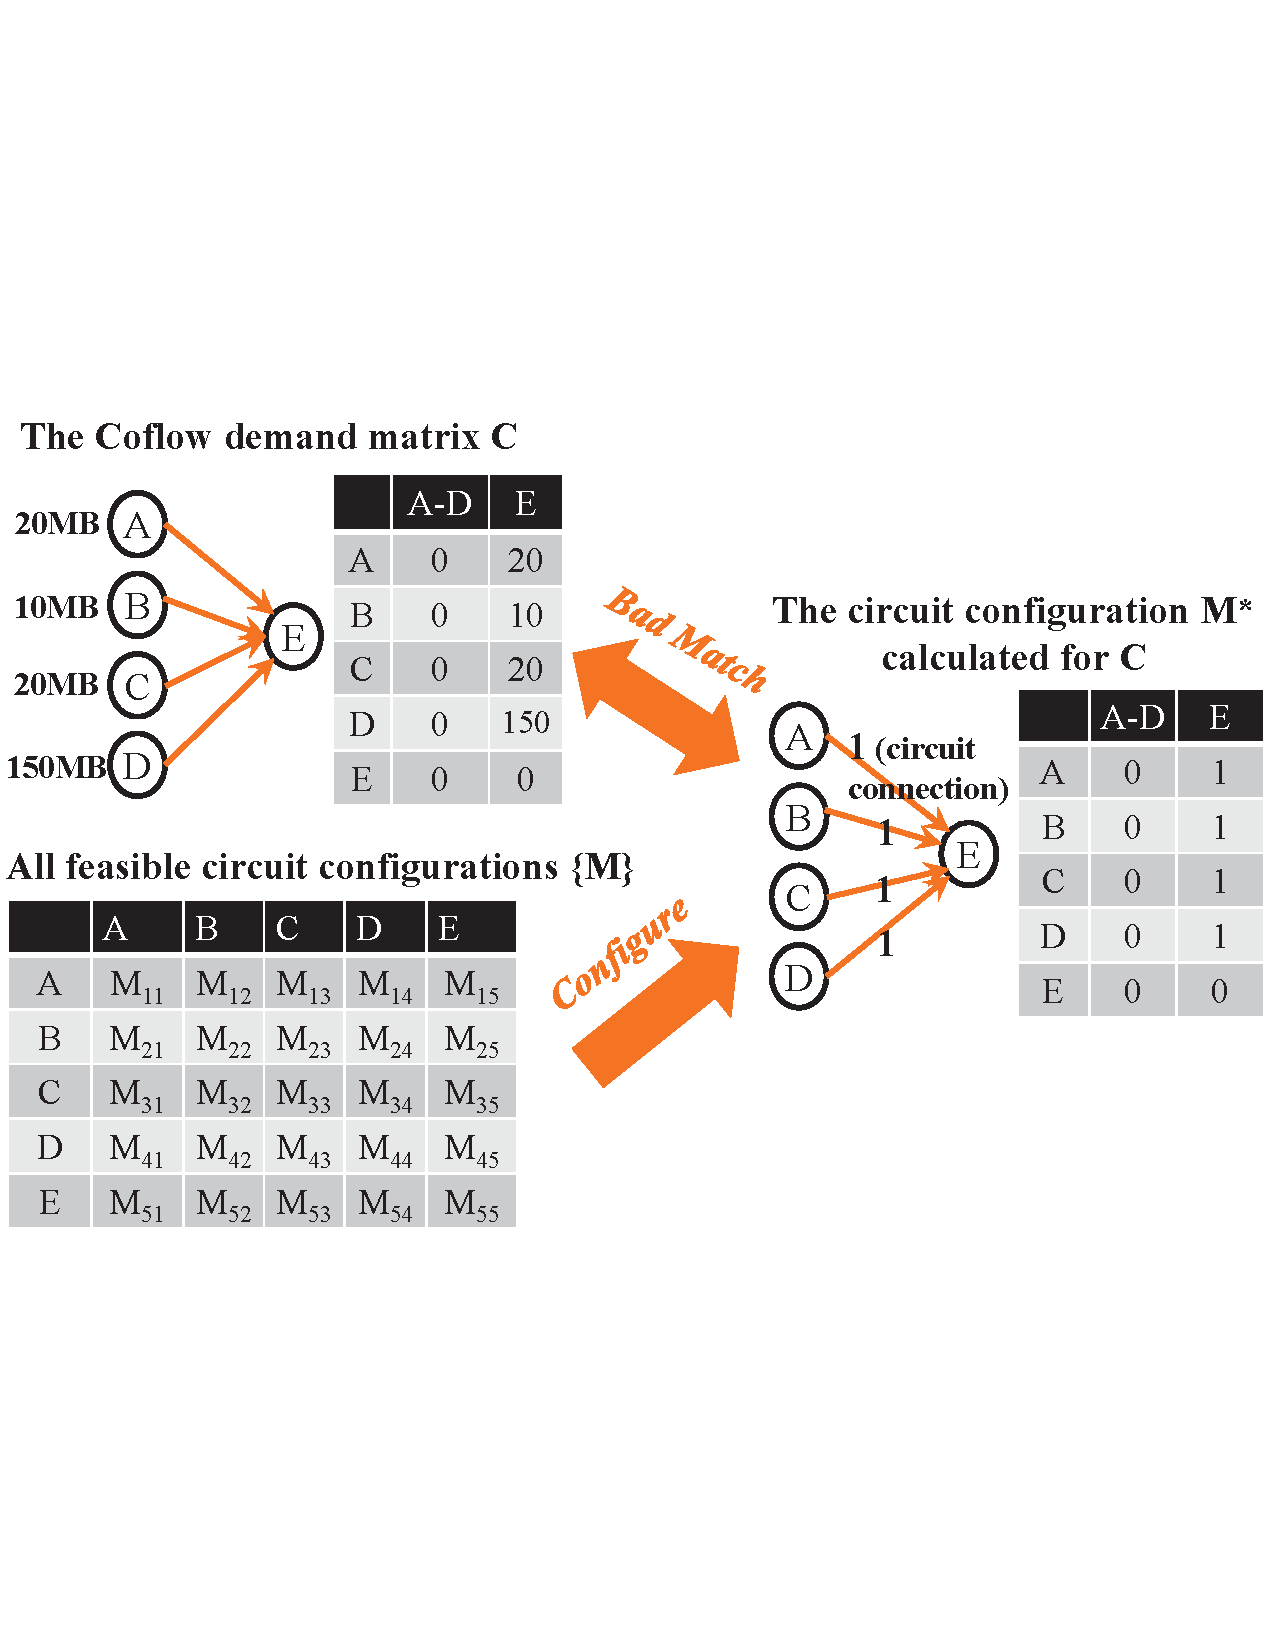
\includegraphics[scale=0.38]{figures/X11}%
  \caption{[Example 1] Circuit configuration $M^*$ calculated via circuit shaping (Problem \ref{problem:1}) cannot well match the coflow demand matrix $C$. We can see that ToR pair $(D,E)$ has 150MB demand while it is only assigned 1 circuit. Such bottleneck pair leads to a CCT of 150$ms$ (calculated by Eq~\eqref{equ:1}), which is 3$\times$ the optimal CCT in packet switched networks (calculated by Eq~\eqref{equ:2}).}
  \label{fig:1}
\end{figure}

\subsection{Shaping the Circuit}
\label{sec:alg1}
Similar to most existing circuit scheduling algorithms, we first try to efficiently configure the circuit to match the coflow traffic pattern.
This directly translates to the following circuit shaping problem:
\begin{problem}
\label{problem:1}
(The circuit shaping problem) Given a coflow demand $C$ and a set of feasible circuit configurations $\{\mathbf{M}\}$, find a configuration $M^* \in \{\mathbf{M}\}$ that minimizes the CCT.
\end{problem}
Note that the CCT can be calculated as
\begin{equation}
CCT = \max\limits_{i,j}(\frac{C_{ij}}{M_{ij}\cdot B})
 \label{equ:1}
\end{equation}
The optimal solution to Problem~\ref{problem:1} can be obtained by first connecting all pairs $(i,j)$ with $C_{ij}>0$, and then iteratively adding connections to the pair $(i^*,j^*)$ with the longest completion time.

However, we find that even with a rich port count, the optimal CCT achieved via circuit shaping can be far from the optimal CCT achievable in packet switched networks.
To illustrate this, consider the example in Figure \ref{fig:1}.
The optical network contains 5 ToRs, each with 4 sending/receiving ports. Each inter-port connection carries a fixed capacity of 1GBps.%\footnote{We use ``Bps" instead of ``bps" to simplify the calculation.}
The coflow demand $C$ follows a many-to-one pattern.

We first calculate the optimal CCT achievable in packet switched networks with the same ingress/egress capacity per ToR. Note that this serves as the lower bound of the CCT achievable in the optical network. In such case, the CCT is constrained only by the ToR with the largest ingress/egress data volume, more specifically we have
\begin{equation}
CCT^{OPT} = \max\bigg(\max\limits_{i}\frac{\sum_jC_{ij}}{B\cdot k}, \max\limits_{j}\frac{\sum_iC_{ij}}{B\cdot k}\bigg)
 \label{equ:2}
\end{equation}
where $B\cdot k$ is the total egress/ingress capacity per ToR. For coflow $C$ in Figure \ref{fig:1}, a CCT of 50$ms$ can be achieved by allocating the 4GBps ingress capacity of ToR $E$ among senders $A$ to $D$ proportionally to their demand.

Compared to the rate allocation that can take any fractional value,
the circuit configuration $M_{ij}$ can only be integers.
For example, a sender can arbitrarily share its egress capacity among different receivers in packet switched networks; in optical networks, however, there is no way to split one sending port into two halves and connecting them to two receiving port simultaneously.
Such integrality constraints result in mismatches between coflow demands and circuit configurations.
On the one hand, ToR pairs with small traffic demand are over-provisioned and can hardly utilize the capacity assigned to them.
In Figure \ref{fig:1}, although ToR pair $(A,E)$ only has a 20MB traffic demand, we still have to establish a circuit connection for it.
As a result, the traffic demand of $(A,E)$ is satisfied after 20$ms$, and the circuit then becomes idle for the rest of the time.\footnote{The connection can be reconfigured after the demand is satisfied if we relax the no-reconfiguration model. However, such reconfiguration still leads to low circuit utilization by introducing large reconfiguration delay (\ie, $\sim$20$ms$ in \cite{megaswitch}). }
On the other hand, ToR pairs with high traffic demand suffer from under-provisioning, which greatly increases the CCT.
For example, ToR pair $(D,E)$ has a 150MB demand, but it is only assigned with one connection and takes 150$ms$ to complete.
Because \emph{a coflow finishes only after all the traffic demand is served}, $(D,E)$ becomes the bottleneck and increases the CCT to 150$ms$.

\begin{figure}[t]
  \centering
  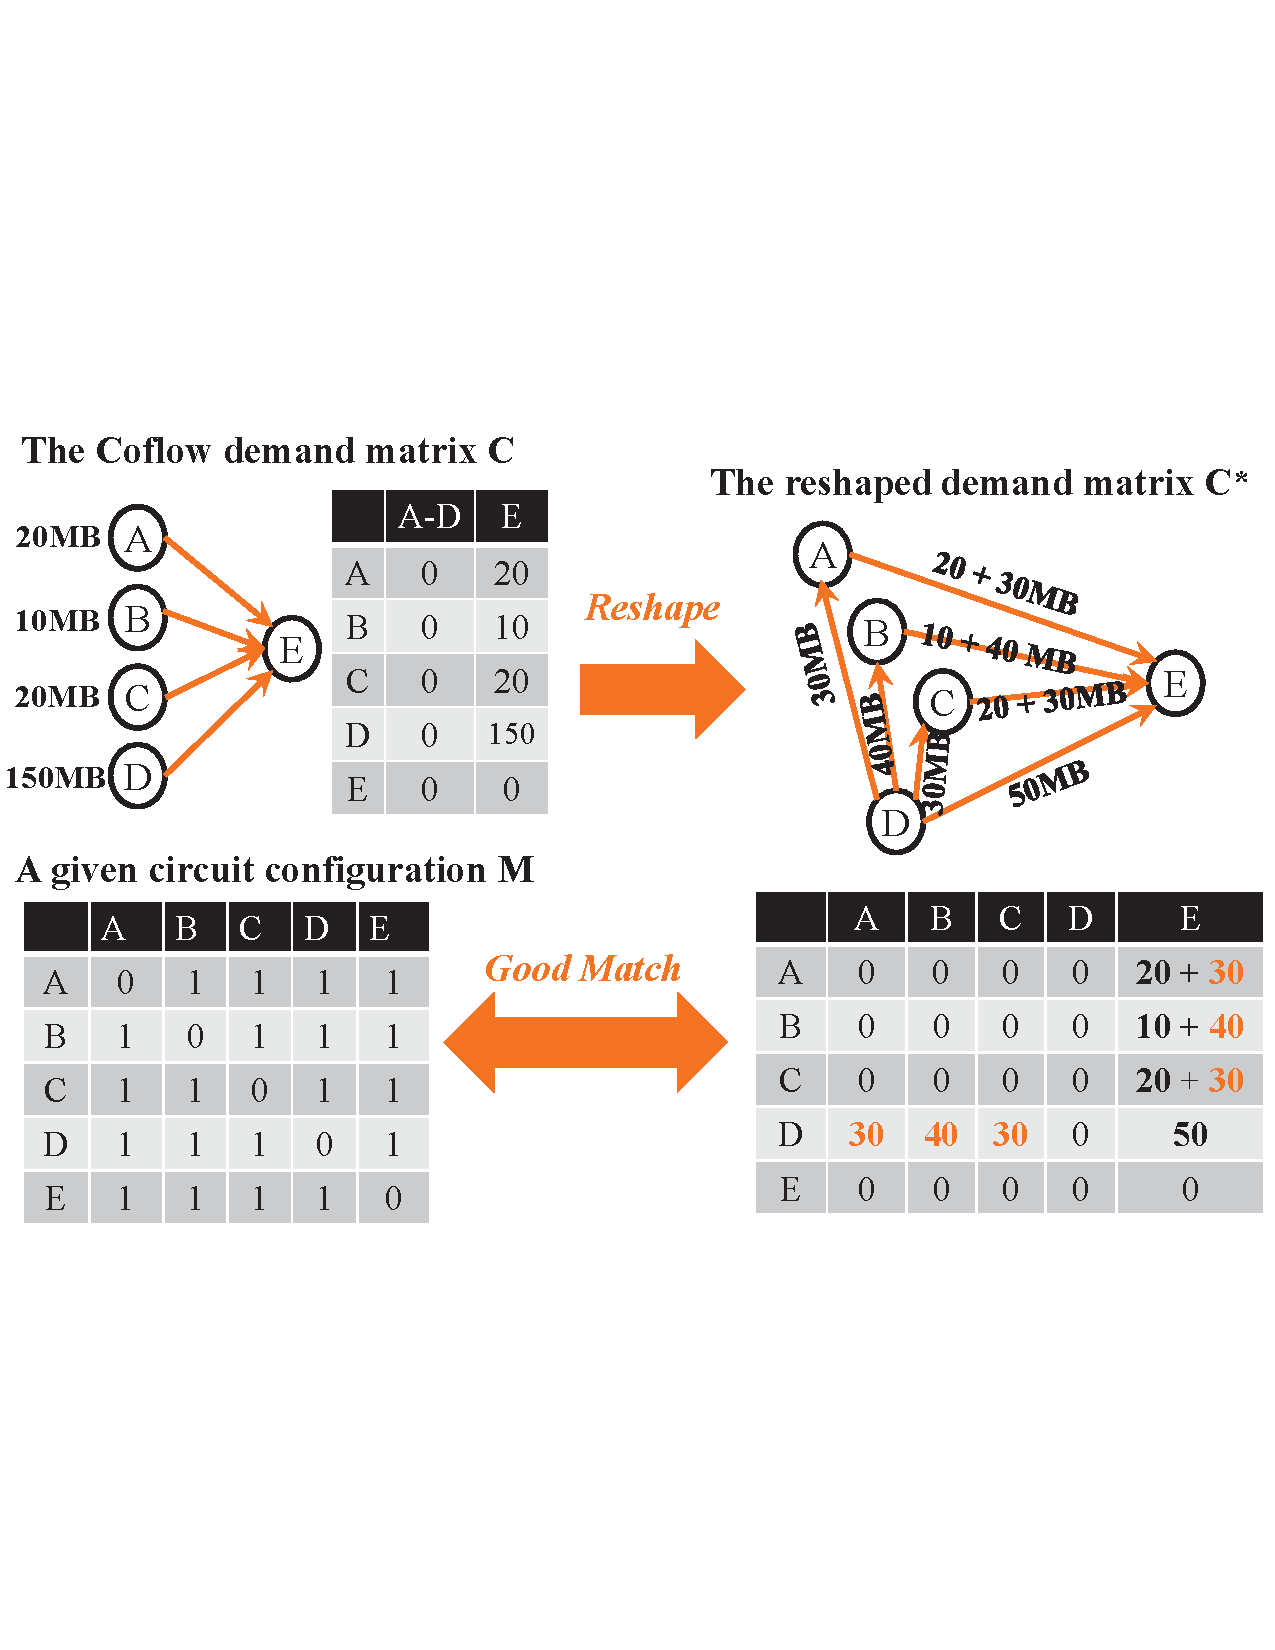
\includegraphics[scale=0.38]{figures/X22}%
  \caption{[Example 2] Given a full-mesh circuit configuration $M$, we can reshape the coflow demand $C$ to $C^*$ to well match the configuration via coflow shaping (Problem \ref{problem:2}). We achieve a CCT of 50$ms$ following this schedule (calculated by Eq~\eqref{equ:1}), which is identical to the optimal CCT in packet switched networks. }
  \label{fig:2}
\end{figure}


\subsection{Shaping the Coflow}
\label{sec:alg2}
To address such mismatch, we explore in the reverse direction and try to reshape the traffic demand matrix to match the circuit configuration.
Following this idea, we leverage multi-hop routing to reshape the traffic demand.
Unlike previous work \cite{osa} that employs multi-hop routing to provide overall connectivity among ToRs, we leverage multi-hop routing to reshape the traffic demands to better match the circuit configuration.
Also, note that the multi-hop routing is done in a cut-through way via source routing, rather than in a store-and-forward manner \cite{eclipse}. Doing so avoids circuit reconfiguration and extra buffer demand.
Specifically, the reshaping is composed of a set of deliberate routing schemes to redistribute the original coflow traffic demand among ToRs.
%fine-grained,

Figure \ref{fig:2} illustrates the effectiveness of such reshaping.
Given a circuit configuration $M$ which forms a full-mesh connection, we can reshape the coflow $C$ to match the configuration $M$.
More specifically, consider the bottleneck ToR pair $(D, E)$ with 150MB demand.
We can effectively resolve it by rerouting these traffic through relaying nodes $A$, $B$ and $C$.
By doing so, we are actually reshaping the traffic demand from $C$ to $C^*$.
We can see that the schedule in Figure \ref{fig:2} results in a CCT of 50$ms$, which is identical to the best solution in packet switched networks.

Formally, we define coflow shaping as follows:
\begin{problem} (The coflow shaping problem)
\label{problem:2}
Given a coflow demand $C$ and a fixed circuit configuration $M$, determine the $C^*$ which can be reshaped from $C$ by multihop routing, so that the CCT (by Eq~\eqref{equ:1}) is minimized.
\end{problem}
We further translate this problem into the multi-commodity flow problem \cite{introduction}, where each ToR pair $(i,j)$ corresponds to a commodity in the multi-commodity flow problem with demand $C_{ij}$.
The goal is to maximize $z$, so that at least $z$ percent of each demand is transferred within a unit time.
Note that CCT equals $1/z$, and the problem can be solved in polynomial time using LP or fast approximation algorithms.

However, coflow reshaping also suffer from major drawbacks.
First, it is not always possible to approach the optimal CCT via coflow reshaping given an arbitrary configuration.
For example, if the circuit connection forms two closed cycles: $(A\rightarrow B, B\rightarrow C, C\rightarrow A)$ and $(D\rightarrow E, E\rightarrow D)$, then there is no way to satisfy the coflow demand via coflow reshaping.
As a result, the effectiveness highly depends on the underlying circuit configuration.
Moreover, notice that multi-hop connection may also result in an inefficient use of the circuit. As we see in Figure \ref{fig:2}, 100MB traffic goes through two-hop paths. As a result, these traffic takes network resource which can potentially serve 200MB traffic demand via direct connection. Such low efficiency may result in reduced goodput and enlarged CCT in the multi-coflow case.

\parab{Implementation Feasibility}
Enabling fine-grained traffic reshaping requires flow-level routing enforcement. We find source routing a good candidate, which pre-installs all the routing rules needed on the ToR switches and does not require the costly dynamic routing table configuration. Specially, we restrict the pre-installed paths to have a hop count less than a threshold $p$.\footnote{This constraint is also considered when calculating the coflow shaping.}
These paths are desirable because of their short lengths, and such restriction greatly reduces the number of routing entries needed.
Note that the coflow demand between a ToR pair often consists of many TCP connections; thus we can distribute these flows over the desirable paths to match the coflow reshaping plan accordingly.

\begin{figure}[t]
  \centering
  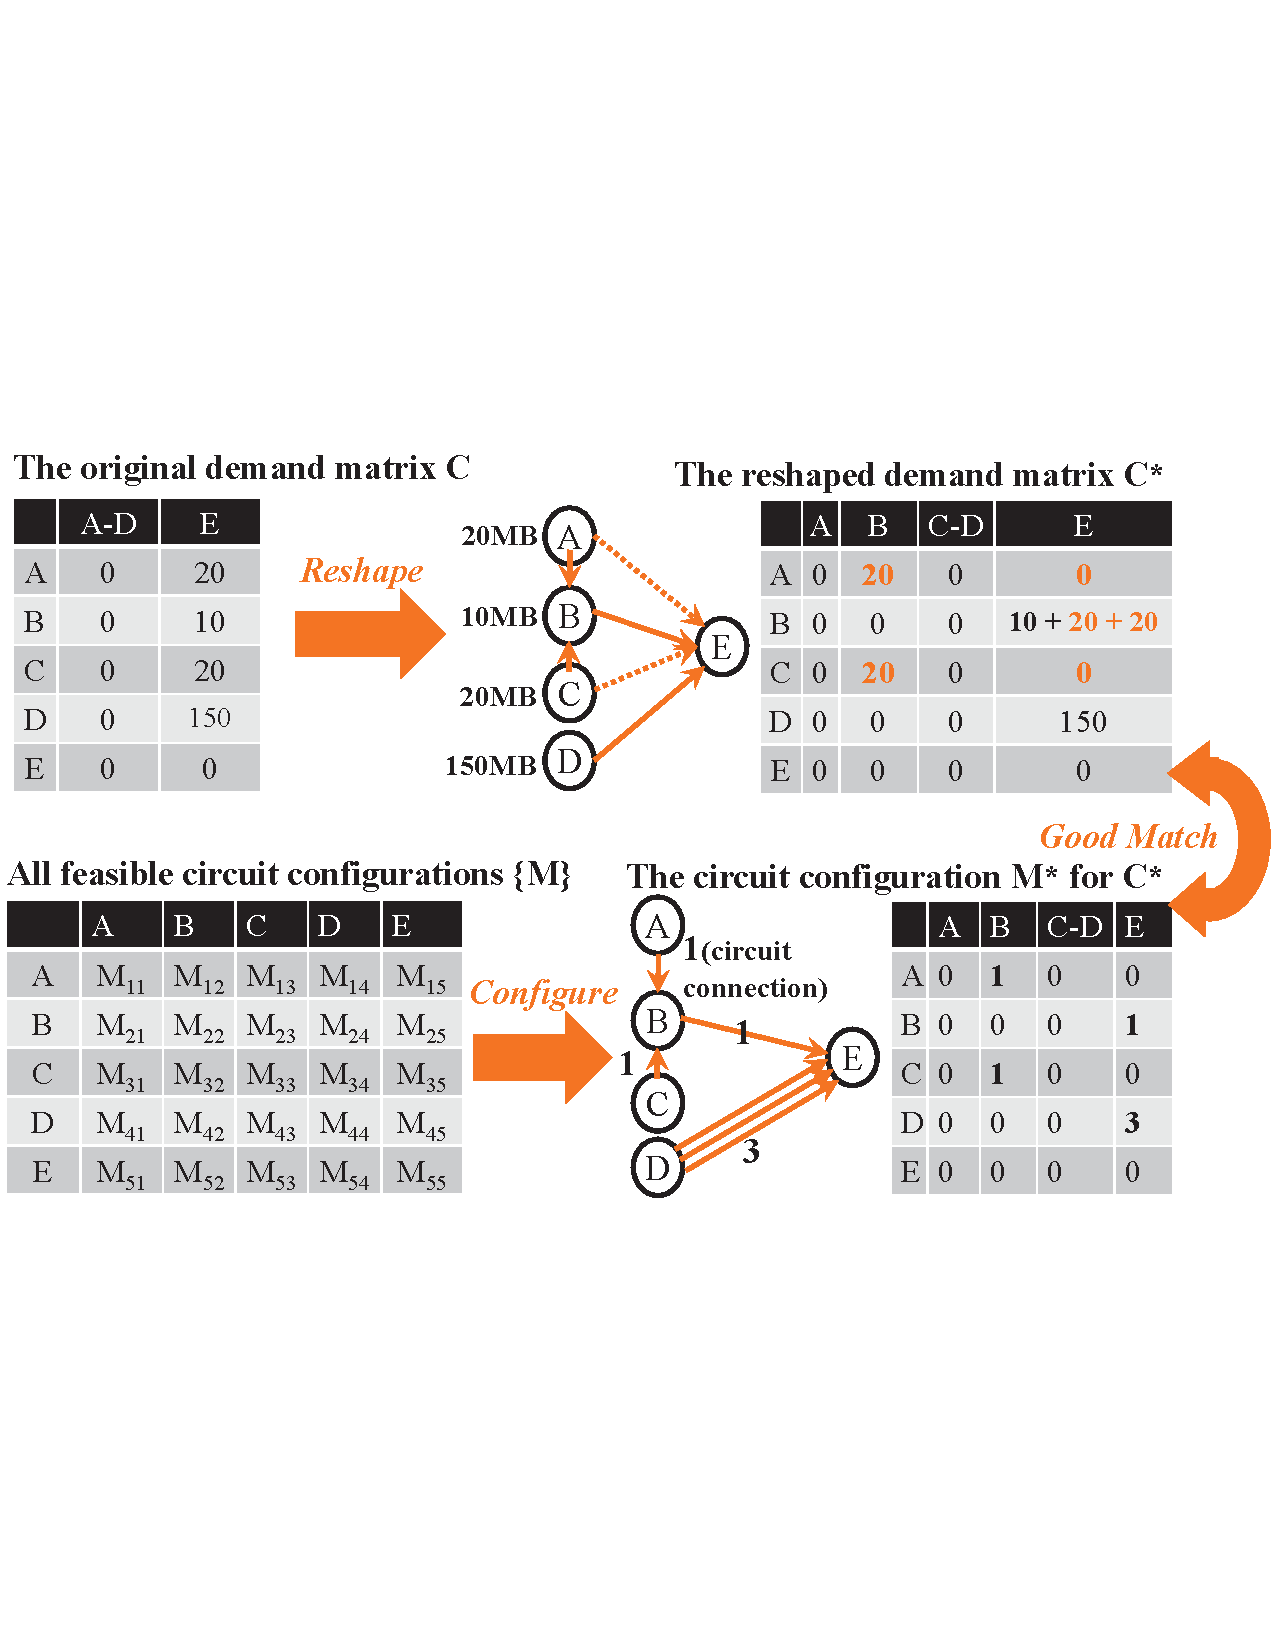
\includegraphics[scale=0.38]{figures/X33}%
  \caption{[Example 3] In joint shaping (Problem \ref{problem:3}) we shape both the circuit $M^*$ and the coflow $C^*$ to match each other.
  We achieve a CCT of 50$ms$ following this schedule (calculated by Eq~\eqref{equ:1}), which is identical to the optimal CCT in packet switched networks. And it introduces much less multi-hop traffic compared to Example \ref{fig:2}.}
  \label{fig:3}
\end{figure}

\subsection{Shaping the Circuit and Coflow Together}
\label{sec:alg3}
Given that neither coflow nor circuit shaping alone can efficiently solve the problem, we focus on jointly shaping both circuit configuration and coflow traffic demand.
More formally, we redefine the coflow scheduling problem as the following joint shaping problem:
\begin{problem} (The joint shaping problem)
\label{problem:3}
Given a coflow demand $C$ and a set of feasible circuit configurations $\{\mathbf{M}\}$, determine the $C^*$ which can be reshaped from $C$ by multi-hop routing and the configuration $M^* \in \{\mathbf{M}\}$, so that the CCT (by Eq~\eqref{equ:1}) is minimized.
\end{problem}

As the example in Figure \ref{fig:3} shows, joint scheduling brings extra flexility to find a good match.
Compared to circuit shaping, joint shaping is not constrained by the integrality constraint.
Compared to coflow shaping, the effectiveness of joint shaping is not constrained by the given circuit configuration.
Moreover, such flexibility also enables more efficient utilization of network resources. As we see in Figure \ref{fig:3}, we achieve the optimal CCT of 50$ms$ while introducing much less multi-hop traffic compare to coflow shaping (Figure \ref{fig:2}).

\begin{algorithm}[!t]
\small
\caption{Heuristic for the Joint Shaping Problem}
\label{ALG-1}
\begin{flushleft}
\textbf{Input:} {$M$: the initial circuit configuration calculated by the circuit shaping;
$C$: the initial coflow demand matrix;
}\\
\textbf{Output:} {$C^*$: the reshaped coflow demand matrix (with the corresp- onding routing scheme);
$M^*$ the updated circuit configuration;}
\end{flushleft}
\begin{algorithmic}[1]
\label{algr:1}
\Procedure{Main}  {}
\State $M^*$ = $M$, $C^*$ = $C$;  \Comment{Initialization;}
\While {true} \Comment{Iteratively resolving the bottleneck;}
%\Procedure{CoflowExtension}{(Identified) Coflows $\mathbb{C}$, diameter $d$}
   \State Calculate the CCT and Identify the bottleneck pair $(s, d)$.
   \State Release\_from\_S($C^*,M^*,CCT$): Release a sending port of $s$;
   \State  Release\_towards\_D($C^*,M^*,CCT$): Release a receiving port of $d$;
  \If {both the above subroutines return true}
        \State $M^*_{sd} = M^*_{sd}+1$; \Comment{Add one link for pair  $(s, d)$ by connecting the released two ports;}
        \State Reshape coflow demand matrix $C^*$ accordingly;
       \Else
       \State \textbf{Return} $M^*$ and $C^*$;
	\EndIf
\EndWhile
\EndProcedure
%\item[]
\Procedure{Release\_from\_S}{$C^*,M^*,CCT$}
%    \While {Fabric is not saturated}
      \State \textbf{Select} the currently least loaded link $(s,u)$ from ToR $s$;
\State  \textbf{From} all the destination ToRs from $s$:
\State \textbf{Select} a relay node $r$ which minimizes $T = \max\big((C_{sr}+C_{su})/(M_{sr}\cdot k), (C_{ru}+C_{su})/(M_{ru} \cdot k)\big)$
\Comment{Shift the load of $(s,u)$  to \big($(s,r)$, $(r,u)$\big) via the least loaded relay node $r$;}
\If {$T<CCT$}  \Comment{Determine if reshaping reduces CCT}
\State \textbf{Return} true;
\EndIf
\EndProcedure
%\item[]
\Procedure{Release\_towards\_D}{$C^*,M^*,CCT$}
\State Done in a similarly way as Release\_from\_S().
\EndProcedure
\end{algorithmic}
\end{algorithm}

However, solving the joint shaping problem is non-trivial because the reshaping of demand matrix $C$ and  circuit configuration $M$ should be tightly coupled.
We design a heuristic that effectively calculates the joint scheduling by
iteratively:
(i) releasing under-utilized circuits by reshaping the coflow demand; and
(ii) configuring the released circuits to serve the bottleneck source-destination ToR pair.
We now describe the main idea by using Example \ref{fig:3}.
We start from the configuration resulted from the circuit shaping problem ($M$ in Figure \ref{fig:1}) and identify the bottleneck ToR pair that determines the CCT ($(D,E)$ in Figure \ref{fig:1}).
We then try to release the under-utilized connections which share the same sender/receiver with the bottleneck ToR pair (connection $A\rightarrow E$ in Figure \ref{fig:1}).
This can be done by rerouting the traffic on these under-utilized connections via multi-hop paths composed of other under-utilized links (reshape the demand $(A, E)$ to $(A, B)$ and $(B, E)$ as shown in Figure \ref{fig:3}).
After that, we assign the released ports to the bottleneck ToR pair (add an extra connection from $D$ to $E$) so that the CCT is reduced.
We run the above procedure iteratively until the CCT cannot be reduced anymore.
Algorithm \ref{ALG-1} describes this in more detail.





% And for routing enforcement, one easily implementable way is to adopt source routing. Specially, we can limit the number of paths





%and restricting routing on these greatly reduces the
% pre-install routing rules for multi-hop paths into the
%corresponding ToR switches, thus no further dynamic
%reconfiguration is needed.





\ignore{
Any distributed rate limiting solutions (\eg,  Hierarchical Token Bucket) can
be applied for practical rate enforcement.


 Idea: more efficiently utilize the bandwidth of the bottleneck, thus minimizing the CCT.

 Release under-utilized links by multi-path traffic grouping.

 An intuitive way to reshape the traffic demand matrix is to
 Following this idea, we leverage the multi-hop relaying

as we can see in the xxx, ....

More formally, we
%given the demand matrix of a coflow $C_1$, we can come up with a rate allocation scheme (represented as a matrix $M$) since the rate assignment is flexible to be any fractional number; the CCT is bounded only by the bottleneck egress/ingress port:

%While under the circut switching model

%Perfect matching from coflow structure to a topology
%Fractional just as the rate assignment
%However wavelength can only be 0-1;
%The bottleneck now is the (src, dst) pair rather than the egress/ingress, due to the integrality wavelength constraint


Optical network with 4 1Gpbs wavelength (4Gbps egress/ingress capacity):
Note that it supports all to all communication;
CCT = max_{all the src,dst pairs}(demand/wavelength*1Gbps) = 3s (under some assumptions)
Can be severe under a biased  demand.


We see that compared to the optimal (fractional) solution, the key problem is that the bottleneck ingress port suffers from a low utilization

The bottleneck ingress port in the optimal solution only has a very low utilization in the optical case with 0-1 assignment.
Thus CCT is enlarged compared to the opt one


Idea: give the bottleneck (src,dst) pair more bandwidth!
How? Release under-utilized links by multi-path traffic grouping.

Idea: more efficiently utilize the bandwidth of the bottleneck, thus minimizing the CCT.
Group and reroute the under-utilized s-d pairs to the bottleneck node.
Now CCT = 3GB/3GBPS =1s
Following this idea, I designed a simple heuristic solution that iteratively minimizing the finishing time of the bottleneck pair by traffic grouping.

In some sense, using multipath is identical to that we changed the demand matrix of the coflow
Well it is essentially restructuring the demand matrix (coflow structure) to minimize the integrality gap

Given coflow demand matrix C and the set of all feasible topology {M}, determine a C’ (by restructuring) and M* \in {M},
   so that  CCT = C’ ./M* is minimized.
Since C’ and M* has many choices, there can be multiple optical (C’, M*);

A heuristic solution.


We can easily extend this ...
The crux here is that




Regarding this question, our first observation is that even with the ability of all-to-all connection, there still exists a gap ....
As

Input: $M$: the initial circuit configuration  calculated by the circuit matching;
$C$: the initial coflow demand matrix
Out: (i).the reshaped coflow demand matrix $C*$ (together with the corresponding routing scheme);  (ii). the new circuit configuration $M*$;

$M*$ = $M$, $C*$ = $C$;  \%initialize

While(1)
Calculate the CCT and Identify the bottleneck pair $(S, D)$.
Release_from_S($C*,M*,CCT$): Release a sending port of $S$;
Release_towards_D($C*,M*,CCT$): Release a receiving port of $D$;
If both the above subroutine return true
$M*_{SD} = M*_{SD}+1$ \%add one link for pair  $(S, D)$ by connecting the released two ports.
Reshape coflow demand matrix: $C*$ accordingly;
else
Return $M*$ and $C*$



Release_from_S($C*,M*,CCT$)
Select the currently least loaded link $(S,U)$ from $S$;
From all the destination ToRs from $S$:
Select a relay node $R$ which minimizes: T = $max(C_{SR}+C_{SU}/M_{SR}, C_{RU}+C_{SU}/M_{RU})$
\%shifting the load of $(S,U)$  to $(S,R)$, $(R,U)$  to the least loaded relay node $R$;
If T < CCT  \%reshaping reduces CCT
Return true;

Release_towards_D
Release a receiving port of D in a similar way

If the CCT’ ) CCT, return the current configuration, otherwise use the relay and continue.

We find a
Given a traffic matrix, find a configuration P* so that Coflow $C_1$ can finish without any reconfiguration.

Especially for xxx that all-to-all


Problem formulation:

The integrality gap
skew

The resulting problem example
The intruisic reason

The solution

Why it is bad, there is a gap

Lower bound of the CCT

How to approach this ?

how to solve this gap?

a reformulation of the problem

Demonstrate the problem
Point out the key to solve the problem and
Formulation
Point out the solution space (properties) given the formulation, which makes two propositions

Then a heuristic

We start by studying how we can optimize the CCT for one single coflow under a fixed topology (\ie with no circuit reconfiguration). %We then extend our ... to the more general case with dynamic arrival/departure of multiple coflows.

To do so, our first attempt is to efficiently shape the circuit to fit the coflow demand.
 %which is then formulated as a circuit matching problem.
However our observation indicates that it is not always possible to come up with a circuit configuration that well matches the coflow demand, and such mismatch results in a CCT far from optimal.

We then explore the reverse direction %, and propose the coflow matching problem which tries to
and try to shape the coflow demand to fit the circuit configuration.
Our analysis demonstrates the feasibility of reshaping the coflow demand matrix by multi-hop routing.
However we also find that the effectiveness of such reshaping highly depends on the underlying circuit configuration.
%We formulate it as a coflow matching problem and translate it into the multi-commodity flow problem.

Such fine-grained scheduling with traffic reshaping is the key advantage over previous solutions, however


Finally, given that neither coflow/circuit shaping along efficiently minimizes CCT, we formulate a joint mapping problem by combining both two designs, and solve it with a simple heuristic algorithm.

%The xxx and xx are then used as subroutines in the most general case with dynamic arrival/departure of multiple coflows.


The general case

where the

What is new ?

In Amoeba, we leverage XPath [11], a simple and readilydeployable
way to implement explicit path control. First,
the XPath manager (which is integrated into the Amoeba
controller) explicitly identifies each desired end-to-end path
with a path ID (in the format of a 32-bit IPv4 address), and
compresses these IDs into IP LPM (Longest Prefix Match)
tables. These routing tables are then pre-installed into the
corresponding inter-DC switches, thus no further dynamic
reconfiguration is needed. Second, each site broker maintains
a path-to-ID mapping table, and translates the routing decision
(made by the controller) into the corresponding path IDs for
each request. Finally, given the path IDs, we leverage NAT at
each sender end-host to translate the raw destination IP into
the desired path ID for each packet, thus explicitly specifies
the routing path


, we can enforce it by enforced by either (i). dynamically updating routing rules on the ToR switches, (ii). pre-configure most multi-hop paths \footnote{We can restrict paths to transverse at most $h$ hops, this greatly reduces the number of paths we need to pre-configure for source routing.} and enforce the routing rules via source routing.

enforcement to realize the decision made by the controller.

for practical rate enforcement
}




\input{sections/NSDI/sched.tex}
%\input{sections/hotnets/simulation.tex}
\input{sections/NSDI/simuNSDI.tex}
%%\vspace{-0.06in}
\section{Related Work}
\vspace{-0.06in}
\parab{Coflow Scheduling in Packet Switched Networks}
Most existing coflow schedulers are designed for packet switched networks \cite{varys,aalo,coda}, while the optical fabric brings two major challenges. First, the circuit configuration introduces the integrality constraint, which serves as the major cause of the mismatch between coflow demand and circuit configuration as we show in Section \ref{sec:alg1}.
Moreover, since reconfiguration introduces non-negligible delay in optical networks, the scheduler has to decide whether to reconfigure the circuit after coflow arrival/departure. As shown in Section \ref{sec:alg4}, this greatly enlarges the solution space and complicates the problem.

\parab{Circuit Scheduling}
%As we mentioned in Section \ref{sec:intro}, the scheduling problem we study greatly differs from the previous circuit scheduling works in terms of traffic pattern, application semantics and connectivity. So
We discuss several most related work in circuit scheduling.
Sunflow \cite{sunflow} first studies the coflow scheduling problem in optical networks. However, it adopts the assumption that one ToR can only establish one connection simultaneously, which no longer holds in many current optical architecture designs \cite{megaswitch,projector}. %Such rich connectivity makes a big difference as we shown in .
Moreover, Sunflow only leverages circuit shaping, which is not sufficient with rich connection among ToRs. Third, preemption is not allowed in Sunflow once the circuit is established. However we notice that it plays an important role in minimizing CCT for multiple coflows ($\S$\ref{sec:alg4}).
%However as we show in Section \ref{sec:alg}, a joint reshaping is important for efficient scheduling with rich connection among ToRs. Third, preemption is not allowed in Sunflow once the circuit is established for a flow. While we notice that preemption (in terms of both circuit configuration and coflow ordering) plays an important role in minimizing CCT for multiple coflows, and we include preemption decisions as important components in our framework ($\S$\ref{sec:alg4}).
Eclipse \cite{eclipse} also leverages multi-hop routing for circuit scheduling, however it
does not consider application semantics such as coflow. Moreover, Eclipse requires the relaying ToR to buffer the traffic and transmit in a subsequent configuration for multi-hop routing.
Doing so requires huge extra buffer and adds at least one extra reconfiguration delay.
%Compare to such store-and-forward method, we can establish multi-hop routing directly via source routing.
%we can directly establish  multi-hop routing rules via openflow \cite{openflow} or programable switches \cite{p4}.
In one word, neither Eclipse nor Sunflow answers our motivating question, that how we can best serve the application traffic demand in start-of-the-art optical datacenter fabrics.

RotorNet \cite{rotornet} proposes a scalable and low-complexity optical datacenter network design
with a fully decentralized control plane. Unfortunately, the decentralized design cannot be easily extended to perform efficient coflow scheduling. The spatial structure of coflow naturally requires coordinated scheduling, and
decentralized coflow scheduling remains an open problem even in packet switched networks \cite{aalo}.

%\vspace{-0.1in}

%Note that such reshaping is different from existing multi-hop routing solutions in OSA, multi-hop overlay networking
%Comparatively, we can enable such reshaping by dynamically updating routing rules on the ToR switches. For example, a sender can arbitrarily allocates its egress capacity to different receivers in packet switched networks.
%However there is no way to split a sending port into two halves and connect to two receiving port simultaneously in optical networks. 
\input{sections/NSDI/conclusion.tex}

%%\vspace{-0.06in}
\section{Related Work}
\vspace{-0.06in}
\parab{Coflow Scheduling in Packet Switched Networks}
Most existing coflow schedulers are designed for packet switched networks \cite{varys,aalo,coda}, while the optical fabric brings two major challenges. First, the circuit configuration introduces the integrality constraint, which serves as the major cause of the mismatch between coflow demand and circuit configuration as we show in Section \ref{sec:alg1}.
Moreover, since reconfiguration introduces non-negligible delay in optical networks, the scheduler has to decide whether to reconfigure the circuit after coflow arrival/departure. As shown in Section \ref{sec:alg4}, this greatly enlarges the solution space and complicates the problem.

\parab{Circuit Scheduling}
%As we mentioned in Section \ref{sec:intro}, the scheduling problem we study greatly differs from the previous circuit scheduling works in terms of traffic pattern, application semantics and connectivity. So
We discuss several most related work in circuit scheduling.
Sunflow \cite{sunflow} first studies the coflow scheduling problem in optical networks. However, it adopts the assumption that one ToR can only establish one connection simultaneously, which no longer holds in many current optical architecture designs \cite{megaswitch,projector}. %Such rich connectivity makes a big difference as we shown in .
Moreover, Sunflow only leverages circuit shaping, which is not sufficient with rich connection among ToRs. Third, preemption is not allowed in Sunflow once the circuit is established. However we notice that it plays an important role in minimizing CCT for multiple coflows ($\S$\ref{sec:alg4}).
%However as we show in Section \ref{sec:alg}, a joint reshaping is important for efficient scheduling with rich connection among ToRs. Third, preemption is not allowed in Sunflow once the circuit is established for a flow. While we notice that preemption (in terms of both circuit configuration and coflow ordering) plays an important role in minimizing CCT for multiple coflows, and we include preemption decisions as important components in our framework ($\S$\ref{sec:alg4}).
Eclipse \cite{eclipse} also leverages multi-hop routing for circuit scheduling, however it
does not consider application semantics such as coflow. Moreover, Eclipse requires the relaying ToR to buffer the traffic and transmit in a subsequent configuration for multi-hop routing.
Doing so requires huge extra buffer and adds at least one extra reconfiguration delay.
%Compare to such store-and-forward method, we can establish multi-hop routing directly via source routing.
%we can directly establish  multi-hop routing rules via openflow \cite{openflow} or programable switches \cite{p4}.
In one word, neither Eclipse nor Sunflow answers our motivating question, that how we can best serve the application traffic demand in start-of-the-art optical datacenter fabrics.

RotorNet \cite{rotornet} proposes a scalable and low-complexity optical datacenter network design
with a fully decentralized control plane. Unfortunately, the decentralized design cannot be easily extended to perform efficient coflow scheduling. The spatial structure of coflow naturally requires coordinated scheduling, and
decentralized coflow scheduling remains an open problem even in packet switched networks \cite{aalo}.

%\vspace{-0.1in}

%Note that such reshaping is different from existing multi-hop routing solutions in OSA, multi-hop overlay networking
%Comparatively, we can enable such reshaping by dynamically updating routing rules on the ToR switches. For example, a sender can arbitrarily allocates its egress capacity to different receivers in packet switched networks.
%However there is no way to split a sending port into two halves and connect to two receiving port simultaneously in optical networks. 
%\input{sections/conclusion.tex}
\clearpage
\bibliographystyle{abbrv}
\begin{small}
\bibliography{reference}
\end{small}


\end{document}
